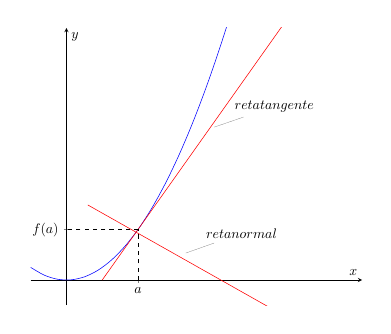
\begin{tikzpicture}[scale=0.5]
\begin{axis}[
 axis lines=middle,
 ticklabel style={fill=white},
%xmin=-1.,%xmax=1.5,
ymin=-0.5, ymax=5,
 xlabel=$x$,ylabel=$y$,
 samples=30,
 smooth,
xtick={1}, ytick={1},
yticklabels={$f(a)$},   xticklabels={$a$},
 width=10cm]
\coordinate  (x2) at (e,1);
\coordinate  (x1) at (0,1);
\addplot[blue, domain=-0.5:5] {x^2};
\addplot[red, domain=0.5:5] {2*x- 1};
\addplot[red, domain=0:5, rotate=-10] {-0.5*x+ 3/2 +0.15};
\node[pin= 30:{$\text{reta tangente}$}] at (axis cs:2,{2*(2)-1}) {};
\node[pin= 30:{$\text{reta normal}$}] at (axis cs:1.6,{-0.5*2+3/2 }) {};
\draw[dashed] (1,0)--(1,1)--(0,1);
\end{axis}
\end{tikzpicture}